%!TEX root = ../trajectory-grouping.tex
Sei $X$ ein topologischer Raum und $f \colon X \to \mathbb{R}$ eine stetige Funktion.
Dann bezeichnet man für einen Wert $a \in \mathbb{R}$ das Urbild unter $f$ als \Index{Niveaumenge} (engl. \emph{level set}) von $a$.
Die Niveaumengen bilden offensichtlich eine Partition von $X$.

Anschaulich stellt man sich $f$ meist als \Index{Höhenfunktion} vor.
So könnte $X$ beispielsweise das Gebiet einer Karte in einem handelsüblichen Atlas sein (= eine Teilmenge der zweidimensionalen Ebene) und $f$ gibt die Höhe über NN an.
Dann sind die Niveaumengen $f^{-1}(\set{a})$ genau die Niveaulinien, die man in detaillierten topografischen Karten findet (ein Beispiel einer solchen Karte findet sich in \cref{sec:karte_niveau}).

Um den \Index{Reeb-Graph} von $f$ zu erhalten, benutzen wir nun die Zusammenhangskomponenten von $f^{-1}(\set{a})$ wie folgt (Definition nach \textcite[\RM{6}.4]{compTopo})

\begin{definition}[{name=[Reeb-Graph]}]
	Der \Index{Reeb-Graph} zu $f \colon X \to \mathbb{R}$ ist der Quotientenraum $\mathcal{R}(f) \coloneqq X/{\sim}$ bezüglich der folgenden Äquivalenzrelation
	\[
		x \sim y \,:\mkern-3mu\iff \exists a \in \mathbb{R} : x,y \text{ liegen in der gleichen Zusammenhangskomponente von } f^{-1}(\set{a})
	\]
	Die Elemente von $\mathcal{R}(f)$ bezeichnen wir als \Index{Konturen} von $f$.
\end{definition}
Wir erhalten eine eindeutig bestimmte Abbildung $h \colon \mathcal{R}(f) \to \mathbb{R}$, sodass das folgende Diagramm kommutiert.
Alle Abbildungen sind aufgrund der universellen Eigenschaft der Quotiententopologie stetig.
\[
	\begin{tikzcd}[sep=large]
		X \rar["f"] \dar["q",two heads] & \mathbb{R} \\
		\mathcal{R}(f) \urar["h"']
	\end{tikzcd}
\]
Die Quotientenabbildung $q$ bildet einen Punkt aus $X$ auf die zugehörige Kontur in $\mathcal{R}(f)$ ab.
% $\mathcal{R}(f)$ ist tatsächlich ein Graph, da jede Niveaumenge unter $q$ auf eine diskrete Menge abgebildet wird.\todo{genauer bzw. expliziter}

Der Reeb-Graph $\mathcal{R}(f)$ beschreibt die Evolution der Konturen (wenn man $\mathbb{R}$ als Zeit interpretiert) und damit wird auch klar, dass $\mathcal{R}(f)$ tatsächlich ein Graph ist, da das Urbild von $a \in \mathbb{R}$ unter $h$ stets eine diskrete Menge von Konturen ist und man $\mathcal{R}(f)$ erhält indem man diese Konturen \enquote{verfolgt}, wobei sie sich sich vereinigen oder aufsplitten können.
Damit muss $\mathcal{R}(f)$ die Struktur eines $1$-dimensionalen CW-Komplexes haben und ist damit insbesondere ein Graph.\footnote{dieser kann allerdings überabzählbar unendlich sein, sofern man keine weiteren Annahmen an $X$ und $f$ trifft}
Betrachtet man die positive Richtung in $\mathbb{R}$, so wird $\mathcal{R}(f)$ auf kanonische Weise zu einem gerichteten Graphen.
Ein Beispiel für einen Reeb-Graphen findet man in \cref{fig:torus_reeb}.

\section{Differentialtopologische Hintergründe zum Reeb-Graphen} % (fold)
\label{sec:background_reeb}
Obwohl wir den Reeb-Graph allgemein definiert haben und auch im weiteren Verlauf keine differenzierbare Struktur auf $X$ benötigen, ist es an dieser Stelle sinnvoll einen kurzen Ausflug in die Differentialtopologie zu machen, um mit einem instruktiven Beispiel zu erläutern, wo genau die Knoten im Reeb-Graphen \enquote{herkommen}.
Neben den gleich auch direkt referenzierten Büchern von \textcite{compTopo} und \textcite{MilnorMorse}, sei an dieser Stelle auf das Buch \citetitle{Miln} von \textcite{Miln} verwiesen, welches einen schnellen, lesenswerten Einstieg in die Grundlagen der Differentialtopologie vermittelt.

Betrachtet man nicht einen beliebigen topologischen Raum $X$, sondern eine differenzierbare Mannigfaltigkeit $M$ wie zum Beispiel den 2-Torus (siehe \cref{fig:torus_reeb}), und eine glatte Funktion $f \colon M \to \mathbb{R}$ so kann man die Punkte von $M$ anhand des Differentials von $f$ in dem jeweiligen Punkt in sogenannte \bet{kritische}\index{kritische Punkte} und \Index{reguläre Punkte} unterteilen.
\begin{figure}
	\centering
	\begin{tikzpicture}[rotate=90, xscale=1, yscale=1, scale=0.7]
		% \draw[help lines] (-4,-10) grid (4,4);
		% reelle Gerade
		\draw[->,thick] (-4,-6) -- ++ (8,0) node[left=3pt]{$\mathbb{R}$};
		
		\draw[DodgerBlue3, thick] (-2.5,1.89) .. controls +(240:0.8) and +(120:0.8) .. (-2.5,-1.89);
		\draw[DodgerBlue3, thick, dashed] (-2.5,1.89) .. controls +(300:0.8) and +(60:0.8) .. (-2.5,-1.89);
		\draw[fill=DodgerBlue3] (-2.5,-6) circle[radius=0.07];
		
		\draw[Firebrick2, thick] (0,2.5) .. controls +(250:0.6) and +(110:0.6) .. (0,0.5);
		\draw[Firebrick2, thick, dashed] (0,2.5) .. controls +(290:0.6) and +(70:0.6) .. (0,0.5);
		
		\draw[Firebrick2, thick] (0,-0.5) .. controls +(250:0.6) and +(110:0.6) .. (0,-2.5);
		\draw[Firebrick2, thick, dashed] (0,-0.5) .. controls +(290:0.6) and +(70:0.6) .. (0,-2.5);
		\draw[fill=Firebrick2] (0,-6) circle[radius=0.07];
		
		\draw[SeaGreen3, thick] (1.75,2.25) .. controls +(250:0.6) and +(110:0.6) .. (1.75,0) .. controls +(250:0.6) and +(110:0.6) .. (1.75,-2.25);
		\draw[SeaGreen3, thick, dashed] (1.75,2.25) .. controls +(290:0.6) and +(70:0.6) .. (1.75,0) .. controls +(290:0.6) and +(70:0.6) .. (1.75,-2.25);
		\draw[fill=SeaGreen3] (1.75,-6) circle[radius=0.07];
		
		\draw[SeaGreen3, thick] (-1.75,2.25) .. controls +(250:0.6) and +(110:0.6) .. (-1.75,0) .. controls +(250:0.6) and +(110:0.6) .. (-1.75,-2.25);
		\draw[SeaGreen3, thick, dashed] (-1.75,2.25) .. controls +(290:0.6) and +(70:0.6) .. (-1.75,0) .. controls +(290:0.6) and +(70:0.6) .. (-1.75,-2.25);
		\draw[fill=SeaGreen3] (-1.75,-6) circle[radius=0.07];
		
		% kritische Werte and Start und Ende
		\begin{scope}
			\clip (-3.5,-1) rectangle (3.5,1);
			\draw[Sienna2,fill=Sienna2] (3.5,0) circle[radius=.08];
			\draw[Sienna2,fill=Sienna2] (-3.5,0) circle[radius=.08];
		\end{scope}
		\draw[fill=Sienna2] (3.5,-6) circle[radius=.07];
		\draw[fill=Sienna2] (-3.5,-6) circle[radius=.07];
		
		% draw reeb graph
		\begin{scope}[every node/.style={shape=circle,inner sep=1.7pt,fill}]
			\draw[thick] (-3.5,-12) node{} -- ++(1.75,0) .. controls +(80:1.5) and +(100:1.5) .. ++(3.5,0) node{};
			\draw[thick] (3.5,-12) node{}-- ++(-1.75,0) .. controls +(-100:1.5) and +(-80:1.5) .. ++(-3.5,0) node{};
		\end{scope}
		\node at (3,-11) {$\mathcal{R}(f)$};
		
		\draw[thick] (-3.5,0) .. controls (-3.5,2) and (-1.5,2.5) .. (0,2.5);
		\draw[thick,xscale=-1] (-3.5,0) .. controls (-3.5,2) and (-1.5,2.5) .. (0,2.5);
		\draw[thick,rotate=180] (-3.5,0) .. controls (-3.5,2) and (-1.5,2.5) .. (0,2.5);
		\draw[thick,yscale=-1] (-3.5,0) .. controls (-3.5,2) and (-1.5,2.5) .. (0,2.5);
		\draw[thick] (-2,.2) .. controls (-1.5,-0.3) and (-1,-0.5) .. (0,-.5) .. controls (1,-0.5) and (1.5,-0.3) .. (2,0.2);
		\draw[thick] (-1.75,0) .. controls (-1.5,0.3) and (-1,0.5) .. (0,.5) .. controls (1,0.5) and (1.5,0.3) .. (1.75,0);
		
		\draw[-to] (0,-3.5) -- (0,-5) node[above, midway]{$f$};
	\end{tikzpicture}
	\caption[Höhenfunktion des aufrechten Torus mit dem dazugehörigen Reeb-Graphen]{Höhenfunktion des aufrechten Torus $T^2=S^1 \times S^1$ mit dem dazugehörigen Reeb-Graphen. Die grün und orange gekennzeichneten Niveaumengen enthalten je einen kritischen Punkt, die rote und blaue enthalten ausschließlich reguläre Werte. $f$ ist eine Morse-Funktion und die Knoten des Reeb-Graphen stehen in Bijektion zu den kritischen Punkten.}\label{fig:torus_reeb}
\end{figure}
Für den aufrechten Torus und die Höhenfunktion sind dies die beiden orange gekennzeichneten, einelementigen Niveaumengen in \cref{fig:torus_reeb}, sowie die beiden \enquote{Klebepunkte} der grün gezeichneten Niveaumengen.

Durch das Betrachten der zweiten Ableitungen in lokalen Koordinaten, kann man die kritischen Punkte anhand der Hesse-Matrix in entartete und nicht entartete einteilen.
Nach \textcite{compTopo} heißt $f$ dann \Index{Morse-Funktion}, wenn
\begin{enumerate}[(i)]
	\item alle kritischen Punkte nicht entartet sind und\marginnote{einige Autoren verzichten auf \cref{enum:def:morse:2}}
	\item\label{enum:def:morse:2} die kritischen Punkte paarweise verschiedene Werte haben.
\end{enumerate}
Beliebige glatte Funktionen $f \colon M \to \mathbb{R}$ lassen sich nach \textcite[Corr.~6.8]{MilnorMorse} gut durch Morse-Funktionen approximieren.

Setze $M^a \coloneqq f^{-1}\enbrace*{(-\infty,a]}$.
Die zentrale Erkenntnis der Morse-Theorie ist es nun, dass sich die Topologie von $M^a$ bei Variation von $a$ nur an den kritischen Werten, also den Bildern kritischer Punkte, ändert.
Darüber hinaus kann diese Änderung als das Ankleben von Zellen realisiert werden.

Für den aufrechten Torus $T$ aus \cref{fig:torus_reeb} ist $T^a$ zum Beispiel zunächst topologisch gesehen eine Scheibe, wird beim Passieren der zweiten kritischen Punktes zu einem Zylinder, beim dritten zu einem Torus, aus dem eine Scheibe ausgeschnitten wurde, und schlussendlich am Maximum zum eigentlichen Torus.

In Bezug auf den Reeb-Graphen bedeutet dies, dass sich auch die Zusammenhangskomponenten der Niveaumengen nur an den kritischen Werten ändern können.
Ein Punkt $u \in \mathcal{R}(f)$ ist also ein Knoten, wenn $q^{-1}(u)$ einen kritischen Punkt enthält.
\Cref{enum:def:morse:2} stellt dann sicher, dass es eine Bijektion zwischen den Knoten im Reeb-Graphen und den kritischen Punkten gibt, die in \cref{fig:torus_reeb} klar ersichtlich ist.
% section background_reeb (end)



\section{Reeb-Graphen zur Gruppierung von Trajektorien} % (fold)
\label{sec:trajek_reeb}
Sei $\mathcal{X}$ wieder eine Menge von Entitäten, die sich entlang bekannter Trajektorien bewegen, die jeweils aus $\tau$ Kanten bestehen.
Indem wir die $z$-Achse des $\mathbb{R}^3$ als Zeit auffassen erhalten wir für jede Entität $x$ durch Extrusion der $\varepsilon$-Scheibe entlang eines Segments der Trajektorie einen schiefen Zylinder im $\mathbb{R}^3$.
Die Vereinigung der $\tau$ Zylinder liefert uns dann einen (ausgefüllten) \enquote{Schlauch} pro Entität, welche wir wiederum alle zu einem Teilraum $\mathcal{M} \subset \mathbb{R}^3$ vereinigen (siehe \cref{fig:tubes}).
Dies ist der Raum, dessen Reeb-Graph wir betrachten wollen.

\begin{figure}
	\centering%
	\subfloat[Der Raum $\mathcal{M}$]{%
	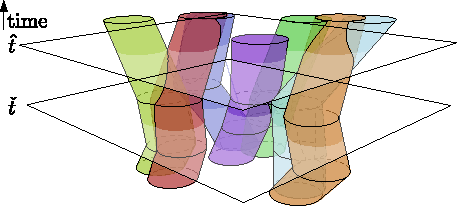
\includegraphics[width=.48\textwidth]{Bilder/manifold_left.pdf}\label{fig:tubes}%
	}
	\hspace{1em}
	\subfloat[Reeb-Graph zu $\mathcal{M}$]{%
	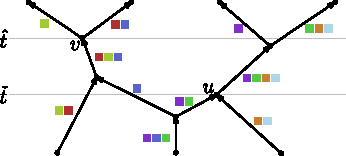
\includegraphics[width=.45\textwidth]{Bilder/manifold_right.pdf}\label{fig:reeb_graph}%
	}
	\caption{Der Raum $\mathcal{M}$ sowie der zugehörige Reeb-Graph $\mathcal{R}$ am Beispiel von sieben Entitäten mit je drei bekannten Positionen, \cite[Fig.~2]{buchin2015}}
\end{figure}

Bezeichnet man nun mit $H_t$ die horizontale Ebene bei der Höhe $t$, so sind die Mengen $\mathcal{M} \cap H_t$ offensichtlich die Niveaumengen.
Eine Zusammenhangskomponente von $\mathcal{M} \cap H_t$ entspricht genau einer Komponente im Sinne von \cref{cha:def_gruppe}, also einer maximalen Menge $\varepsilon$-zusammenhängender Entitäten zum Zeitpunkt $t$.

Der Einfachheit halber nehmen wir im weiteren Verlauf folgendes an:
\begin{itemize}
	\item Die bekannten Positionen der Trajektorien sind alle an gleichen Zeitpunkten $t_0, \ldots ,t_\tau$.
	\item Keine drei Entitäten werden zur gleichen Zeit $\varepsilon$-(un)zusammenhängend.
\end{itemize}
Diese Annahmen können ohne Beschränkung der Allgemeinheit getroffen werden:
Die erste Annahme lässt sich durch das Zerteilen einzelner Segmente der Trajektorien zu geeigneten Zeitpunkten auch leicht künstlich herstellen; in vielen Anwendunsfällen aber wird die Datenerhebung für alle Entitäten direkt zur gleichen Zeit stattfinden.
Die zweite Annahme ist zum einen in nicht explizit als Gegenbeispiel konstruierten Daten sehr unwahrscheinlich und lässt sich notfalls durch weitere Spezialfälle im Algorithmus abfangen.

\begin{definition}[{name=[Reeb-Graph der \GrpStruktur]}]
	Wir bezeichnen mit $\mathcal{R}$ den Reeb-Graphen zu $\mathcal{M}$ bezüglich der Höhenfunktion zu $\mathcal{M}$.
\end{definition}

% In vielen Fällen ist $\mathcal{M}$ eine $3$-Mannigfaltigkeit mit Rand -- wenn zwei Entitäten während eines Zeitabschnittes aber konstant den Abstand $2 \varepsilon$ haben, so ist $\mathcal{M}$ keine Mannigfaltigkeit!
% Wie wir später sehen werden, kann dies im Algorithmus aber als Spezialfall behandelt werden.

An dieser Stelle sei angemerkt, dass $\mathcal{M}$ ein dreidimensionaler Raum ist (bis auf einige wenige Ausnahmen ist $\mathcal{M}$ eine 3-Mannigfaltigkeit mit Rand\footnote{Gegenbeispiel: Zwei Entitäten haben während eines Zeitabschnitts konstant den Abstand $2 \varepsilon$. Im Algorithmus in \cref{cha:berechnung} wird dieser Fall explizit abgefangen.}; in jedem Fall ist $\mathcal{M}$ ein dreidimensionaler CW-Komplex) im Gegensatz zum \emph{zwei}dimensionalen Torus, der eben betrachtet wurde.
Das in \cref{fig:bsp_reeb_rand} betrachtete Beispiel zeigt, warum wir den dreidimensionalen Raum $\mathcal{M}$ und nicht dessen zweidimensionalen Rand betrachten.

\begin{figure}
	\centering
	\begin{tikzpicture}[scale=1.3]
		\foreach \x in {0,30,...,330}{
			\filldraw[Firebrick2] (\x:1) circle[radius=.4];
		}
		\foreach \x in {0,30,...,330}{
			\fill[white] (\x:1) circle[radius=.37];
		}
		\foreach \x in {0,30,...,330}{
			\fill[DodgerBlue3,fill opacity=.5] (\x:1) circle[radius=.37];
			\filldraw (\x:1) circle[radius=.04];
		}
 	\end{tikzpicture}
	\caption[Unterschiede bei den Zusammenhangskomponenten zwischen $\mathcal{M}$ und $\partial \mathcal{M}$]{Angenommen die gezeichneten Entitäten bewegen sich gar nicht. Jede Niveaumenge von $\mathcal{M}$ ist dann zusammenhängend, die Niveaumengen des Randes $\partial \mathcal{M}$ bestehen aber stets aus zwei Zusammenhangskomponenten. Da obige Konfiguration (bei geeignetem $\delta$) nur eine maximale Gruppe bildet, wurde $\mathcal{R}$ als Reeb-Graph von $\mathcal{M}$ und nicht $\partial \mathcal{M}$ definiert.}\label{fig:bsp_reeb_rand}
\end{figure}

Wie in \cref{sec:background_reeb} erläutert, entsprechen die Vertices von $\mathcal{R}$ Zeitpunkten $t_v$, an denen sich die Komponenten ändern.
Diese Zeitpunkte stimmen im Allgemeinen nicht mit den Zeitpunkten $t_0, \ldots, t_\tau$ überein, was auch in \cref{fig:tubes,fig:reeb_graph} zu erkennen ist.

Jeder Vertex im Reeb-Graphen lässt sich nun eindeutig einer der folgenden Klassen zuordnen:
\begin{description}
	\item[Start-Vertex] Für jede Komponente zum Zeitpunkt $t_0$ existiert ein Vertex; ein solcher Vertex ist ein \Index{Start-Vertex}.
	Jeder Start-Vertex hat Eingangs-Grad 0 und Ausgangsgrad 1.
	\item[End-Vertex] Genauso existiert für jede Komponente zum Zeitpunkt $t_\tau$ ein Vertex, ein sog. \Index{End-Vertex}.
	Jeder End-Vertex hat Eingangs-Grad 1 und Ausgangsgrad 0.
\end{description}
Die verbleibenden Vertices können wir aufgrund der Annahme, dass keine drei Entitäten zur gleichen Zeit $\varepsilon$-(un)zusammenhängend werden, eindeutig einer der beiden folgenden Klassen zuordnen: Ein
\begin{description}
	\item[Merge-Vertex] hat Eingangs-Grad 2 und Ausgangsgrad 1, ein
	\item[Split-Vertex] hat Eingangs-Grad 1 und Ausgangsgrad 2.
\end{description}
Eine gerichtete Kante $e=(u,v)$ in $\mathcal{R}$ entspricht einer Menge von Entitäten, die zu jedem Zeitpunkt $t \in \benbrace*{t_u,t_v}$ eine Komponente (im Sinne von \cref{cha:def_gruppe}) bildet.
Wir halten fest, dass der Reeb-Graph $\mathcal{R}$ nur vom räumlichen Parameter $\varepsilon$, aber nicht von den beiden weiteren Parametern unseres Modells, $m$ und $\delta$, abhängt.

Wie genau hängt der Reeb-Graph $\mathcal{R}$ nun mit den Trajektorien und den Gruppen zusammen?
Zunächst einmal folgt jede Entität einem Pfad in $\mathcal{R}$ von einem Start-Vertex zu einem End-Vertex.
Analog lässt sich jeder (maximalen) Gruppe ein Pfad von einem Start- oder Merge-Vertex zu einem End- oder Split-Vertex zuordnen.
Wählt man nun $m > 1$ oder $\delta > 0$, so kann es sein, dass einigen Kanten von $\mathcal{R}$ keine Gruppe zugeordnet ist und sie somit für die \GrpStruktur irrelevant sind.
$\mathcal{R}$ ohne all diese Kanten ist der \Index{reduzierte Reeb-Graph}, den wir ebenfalls mit $\mathcal{R}$ bezeichnen (nur für die Komplexität von $\mathcal{R}$ nehmen wir gleich noch einmal den unreduzierten Fall an).


\begin{definition}[{name=[{\GrpStruktur}]},label=def:grpstrukur]
	Die \bet{\GrpStruktur}\index{Gruppierungsstruktur} (\enquote{trajectory grouping structure}) zu $\mathcal{X}$ und den Parametern $(\varepsilon,\delta,m)$ besteht aus dem reduzierten Reeb-Graphen $\mathcal{R}$ und einer Abbildung, die jeder Kante die zugehörige Menge maximaler Gruppen zuordnet.
\end{definition}
% section trajek_reeb (end)

\section{Komplexität der \GrpStruktur} % (fold)
\label{sec:komplex}
Gemäß \cref{def:grpstrukur} müssen wir sowohl für die Komplexität des Reeb-Graphen $\mathcal{R}$ als auch die Anzahl maximaler Gruppen obere Schranken finden.
Dazu folgen wir \textcite[Sec.~2.1~\&~2.2]{buchin2015} und beweisen Schranken von $\mathcal{O}(\tau n^2)$ für $\abs*{\mathcal{R}}$ und $\mathcal{O}(\tau n^3)$ für die Anzahl maximaler Gruppen, die im Worst-Case sogar scharf sind.

\begin{lemma}[name={\cite[Lem.~1]{buchin2015}},label=lem:untereSchranke-Reeb]
	Der Reeb-Graph $\mathcal{R}$ einer Menge $\mathcal{X}$ von $n$ Entitäten, von denen sich jede auf einer Trajektorie mit $\tau$ Kanten bewegt, kann $\Omega(\tau n^2)$ Vertices und $\Omega(\tau n^2)$ Kanten haben.
\end{lemma}
\begin{beweis}
	Wir nehmen ohne Einschränkungen an, dass $n$ gerade sei; weiter können wir $\varepsilon=0$ wählen.
	Wir wollen nun eine Menge von Trajektorien konstruieren, sodass $\mathcal{R}$ $\Omega(n^2)$ viele Vertices $v$ mit $t_v \in \benbrace*{t_i,t_{i+1}}$ hat für einen der Zeitpunkte $t_i$.
	Diese Konstruktion wiederholen wir für alle Intervalle.
	Dies liefert dann offensichtlich $\Omega(\tau n^2)$ viele Vertices und damit auch $\Omega(\tau n^2)$ viele Kanten, da jeder Knoten entweder Grad 1 oder Grad 3 hat (siehe oben).
	
	Wir teilen $\mathcal{X}$ -- wie in \cref{fig:vertices-intervall} gezeichnet -- in zwei Teilmengen $R= \set{r_1, \ldots ,r_{n/2}}$, $D=\set{d_1,\ldots ,d_{n/2}}$ auf, wobei die Entität $r_j$ bei $(-j,-j)$ und $d_\ell$ bei $(\ell,\ell)$ startet.
	\begin{figure}
		\centering
		\begin{tikzpicture}[scale=.3,>=Latex,font=\small]
			\draw[dashed] (-7,-7) node[left]{$t_i$} -- (7,7);
			\draw[dashed] (0,-12) node[left]{$t_{i+1}$} -- ++ (14,14);
			\foreach \x in {1,2,3,4,5}{
				\draw[->,thick] (-\x,-\x) node[left]{$r_{\x}$} -- ++ (12,0);
				\draw[->,thick] (\x,\x) node[above,xshift=-1pt]{$d_{\x}$} -- ++ (0,-12);
				\filldraw[fill=DodgerBlue3] (-\x,-\x) circle[radius=.15] ++ (12,0)circle[radius=.15];
				\filldraw[fill=Firebrick2] (\x,\x) circle[radius=.15] ++ (0,-12) circle[radius=.15];
			}
		\end{tikzpicture}
		\caption{Konstruktion für $\Omega(n^2)$ viele Vertices im Intervall $\benbrace*{t_i,t_{i+1}}$ am Beispiel $n=5$}\label{fig:vertices-intervall}
	\end{figure}
	Alle Entitäten bewegen sich mit der Geschwindigkeit Eins, die $r_j$ nach rechts, die $d_\ell$ nach unten.
	Aus \cref{fig:vertices-intervall} ist klar ersichtlich, dass sich die Konstruktion mit vertauschten Rollen im nächsten Intervall wiederholen lässt.
	Da sich $r_j$ und $d_\ell$ zum Zeitpunkt $t_i + j + \ell$ treffen, entsteht ein Vertex im Reeb-Graphen und wir erhalten insgesamt $\Omega(n^2)$ Vertices pro Zeitintervall.
\end{beweis}

\begin{satz}[name={\cite[Thm.~2]{buchin2015}},label=thm:schranke-Reeb]
	Der Reeb-Graph $\mathcal{R}=(V,E)$ aus \cref{lem:untereSchranke-Reeb} hat $\mathcal{O}(\tau n^2)$ Vertices und Kanten.
	Diese Schranke ist scharf im Worst-Case.
\end{satz}
\begin{beweis}
	In \cref{lem:untereSchranke-Reeb} wurde bereits eine Konstruktion angegeben, die einen Reeb-Graphen mit $\Omega(\tau n^2)$ Vertices und Kanten liefert.
	Wir müssen also nur noch zeigen, dass höchstens $\mathcal{O}(\tau n^2)$ Vertices und Kanten entstehen können.
	Dazu nutzen wir aus, dass sich die Entitäten während eines Zeitintervalls $\benbrace*{t_i,t_{i+1}}$ auf Geraden bewegen.
	Insbesondere ist nämlich der Abstand zwischen zwei Entitäten $x$ und $y$ während $\benbrace*{t_i,t_{i+1}}$ eine konvexe Funktion $\benbrace*{t_i,t_{i+1}} \to \mathbb{R}_+$, wie man sehr leicht mit Hilfe der Dreiecksungleichung zeigt.\footnote{dabei kann man sogar ganz allgemein eine beliebige Norm auf $\mathbb{R}^d$ betrachten}
	Damit sind $x$ und $y$ höchstens während eines Intervalls $I \subseteq \benbrace*{t_i,t_{i+1}}$ direkt-zusammenhängend.
	Dieses Intervall liefert wiederum höchstens zwei Vertices in $\mathcal{R}$.
	Da die Trajektorien aus je $\tau$ Kanten bestehen, erzeugt jedes Paar $(x,y)$ somit $\mathcal{O}(\tau)$ Vertices.
	Damit gibt es insgesamt $\mathcal{O}(\tau n^2)$ Vertices und damit auch $\mathcal{O}(\tau n^2)$ Kanten, da der Knotengrad beschränkt ist.
\end{beweis}

Da sich die Konstruktion aus \cref{lem:untereSchranke-Reeb} kanonisch in den $\mathbb{R}^d$ einbetten lässt und das Argument mit der Konvexität der Abstandsfunktion in beliebigen Dimensionen funktioniert, gilt \cref{thm:schranke-Reeb} auch für Trajektorien im $\mathbb{R}^d$.

Wir zeigen nun, dass die Anzahl der maximalen Gruppen in $\mathcal{O}(\tau n^3)$ liegt.
Dies gestaltet sich etwas schwieriger als die Komplexität des Reeb-Graphen, da man oftmals erst an einem Split feststellt, dass eine Gruppe maximal ist, auch wenn sie schon vorher begonnen hat.

\begin{lemma}[name={\cite[Lem.~4]{buchin2015}},label=lem:untereSchranke-Gruppen]
	Für eine Menge $\mathcal{X}$ von $n$ Entitäten, von denen sich jede entlang einer Trajektorie von $\tau$ Kanten bewegt, kann es $\Omega(\tau n^3)$ maximale Gruppen geben, wobei jede eine Größe von $\Omega(n)$ hat.
\end{lemma}
\begin{beweis}
	Wir gehen ähnlich wie in \cref{lem:untereSchranke-Reeb} vor, das heißt wir konstruieren $n$ Kanten von Trajektorien für ein Zeitintervall $\benbrace*{t_u,t_{u+1}}$, welche $\Omega(n^3)$ maximale Gruppen mit $I_G \subseteq \benbrace*{t_u,t_{u+1}}$ erzeugen, sodass eine Wiederholung der Konstruktion für alle Zeitintervalle in der gewünschten Anzahl maximaler Gruppen resultiert.
	
	Wir nehmen ohne Einschränkungen an, dass $n$ durch 13 teilbar ist und zerteilen $\mathcal{X}$ in zwei Mengen $S$ und $D$ mit $\abs*{S}=\frac{12n}{13}$ und $\abs*{D}=\frac{n}{13}$.
	Dabei platzieren wir $\frac{8n}{13}$ Entitäten aus $S$ auf der $x$-Achse mit Abstand $r$, wobei $\varepsilon< r < 2 \varepsilon$.
	Oberhalb jeder vierten Entität $s_i$ platzieren wir zwei weitere auch mit dem Abstand $r$, sodass sich ein \enquote{Zinnenkranz} aus Zinnen $T_i$ entsteht (siehe \cref{fig:zinnen}).
	Per Konstruktion hat $S$ $\frac{2n}{13}$ solcher Zinnen und $S$ ist $\varepsilon$-zusammenhängend.
	Die Entitäten aus $S$ bleiben stationär.
	
	\begin{figure}[hbtp]
		\centering
		\begin{tikzpicture}[scale=.5]
			\foreach \x in {1,...,24}{
				\draw[fill=black,fill opacity=.7] (\x,0) circle[radius=.7];
			}
			\foreach \x in {1,2,...,6}{
				\draw[fill=black,fill opacity=.7] ($4*(\x,0) - 3*(1,0) + (0,1)$) circle[radius=.7];
				\draw[fill=black,fill opacity=.7] ($4*(\x,0) - 3*(1,0) + (0,2)$) circle[radius=.7];
				\node at ($4*(\x,0) - 3*(1,0.4)$) {$T_\x$};
			}
			\foreach \x in {1,2,3}{
				\draw[fill=Firebrick2,fill opacity=.7] ($(8,2) - 4.4*(\x,0) + 4.4*(1,0)$) circle[radius=.7] ;
				\node at ($(8,2) - 4.4*(\x,0) + 4.4*(1,0.25)$) {$d_\x$};
			}
			\draw[|-|] (13,3.5) -- ++ (4,0) node[midway,fill=white]{$4r$};
			\draw[|-|] (8,4) -- ++ (-4.4,0) node[midway,fill=white]{$4r + \frac{\varepsilon}{n}$};
		\end{tikzpicture}
		\caption{Konstruktion der unteren Schranke für die Anzahl maximaler Gruppen für $n=39$ zum Zeitpunkt $j_2$ in Runde drei.}\label{fig:zinnen}
	\end{figure}
	
	Die Entitäten in $D$ hingegen bewegen sich auf der Geraden $y=2r$ in gleicher Geschwindigkeit nach rechts, wobei sie zum Zeitpunkt $t_u$ alle links der Scheiben von $S$ liegen und zu $t_{u+1}$ rechts davon.
	Wir nummerieren die Elemente in $D$ von rechts nach links und ihr Abstand soll jeweils $4r + \frac{\varepsilon}{n}$ betragen (siehe \cref{fig:zinnen}).
	
	Die Ereignisse im Intervall $\benbrace*{t_u,t_{u+1}}$ lassen sich nun in mehrere \emph{Runden} einteilen.
	Eine Runde soll dabei die Ereignisse zusammenfassen, die passieren, während $d_1$ eine der \enquote{Zinnen} $T_i$ passiert.
	Eine solche Runde $z$ startet mit $k$ Merge-Ereignissen zu den Zeitpunkten $j_1, \ldots , j_k$ gefolgt von $k$ Split-Ereignissen $\ell_1, \ldots, \ell_k$.
	Genauer wird $d_i$ zum Zeitpunkt $j_i$ $\varepsilon$-zusammenhängend mit $S$ bei $T_{1+z-i}$ und ist es ab dem Zeitpunkt $\ell_i$ nicht länger.
	
	Diese Reihenfolge ist durch die Wahl des Abstandes $4r + \frac{\varepsilon}{n}$ sichergestellt: Damit alle Merge-Ereignisse vor den Split-Ereignissen stattfinden können, müssen alle weiteren an dieser Runde beteiligten Entitäten $\varepsilon$-zusammenhängend mit $S$ werden bevor $d_1$ nicht mehr mit $S$ verbunden ist.
	Beim Passieren legt $d_1$ eine Strecke von $4 \varepsilon$ zurück und nach jeweils $\frac{\varepsilon}{n}$ zurückgelegter Strecke, wird eine der bis zu $\frac{n}{13}-1$ vielen weiteren Entitäten mit $S$ verbunden.
	Da $4 \varepsilon > \enbrace*{\frac{n}{13}-1 } \cdot \frac{\varepsilon}{n}$ gilt, ist nun obige Reihenfolge von Ereignissen gegeben.
	
	\begin{figure}
		\centering
		\begin{tikzpicture}[scale=.5,yscale=.9]
			\pgfmathsetmacro{\height}{10}
			\foreach \x in {1,...,4}{
				\draw[dashed] ($(\x,0) - (1,0)$) node[below]{$j_\x$} -- ++ (0,\height);
				\draw[dashed] ($(\x,0) + (12,0)$) node[below]{$\ell_\x$} -- ++ (0,\height);
				\draw[ultra thick] ($(\x,\height) - (1,0) - 0.7*(0,\x)$) -- ($(13,\height)- 0.7*(0,\x)$);
				\node at ($(-0.8,\height) - 0.7*(0,\x)$) {$G_{1\x}$};
			}
			\foreach \x in {2,3,4}{
				\draw[ultra thick] ($(\x,\height) - (1,2.8) - 0.7*(0,\x)$) -- ++ ($(15,0) - (\x,0)$);
				\node at ($(-0.8,\height) - (0,2.8) - 0.7*(0,\x)$) {$G_{2\x}$};
			}
			\foreach \x in {3,4}{
				\draw[ultra thick] ($(\x,\height) - (1,4.9) - 0.7*(0,\x)$) -- ++ ($(16,0) - (\x,0)$);
				\node at ($(-0.8,\height) - (0,4.9) - 0.7*(0,\x)$) {$G_{3\x}$};
			}
			\draw[ultra thick] ($(4,\height) - (1,9.1)$) -- ++ (13,0);
			\node at ($(-0.8,\height) - (0,9.1)$) {$G_{44}$};
		\end{tikzpicture}
		\caption{Die Zeitintervalle der maximalen Gruppen $G_{ab}$.}\label{fig:gruppen-intervalle}
	\end{figure}
	
	Setze $G_{ab} \coloneqq S \cup \bigcup_{h=a}^b d_h$.
	Jedes Merge-Ereignis startet eine neue maximale Gruppe $G_{1i}$, also sind nach den Merge-Ereignissen $k$ maximale Gruppen entstanden.
	In den darauf folgenden Split-Ereignissen werden $d_1, \ldots , d_k$ nach und nach von $S$ getrennt -- wenn $d_i$ nicht mehr $\varepsilon$-zusammenhängend zu $S$ ist, enden die maximalen Gruppen $G_{ii}, \ldots , G_{ik}$.
	Gleichzeitig werden nun aber die Gruppen, die bei $j_{i+1}$ gestartet sind zu maximalen Gruppen $G_{(i+1)h}$, da $d_i$ die Gruppe $G_{ih}$ verlassen hat (siehe \cref{fig:gruppen-intervalle}).
	
	Dies bedeutet, dass das Ereignis $\ell_i$ genau $k-i$ viele neue maximale Gruppen erzeugt.
	Zusammen mit den $k$ maximalen Gruppen $G_{1i}$ erzeugt die Runde $z$ also
	\[
		\sum_{i=0}^{k} (k-i)  \in \Omega(k^2)
	\]
	viele maximale Gruppen.
	Damit erhalten wir für $m \le \frac{12n}{13}$ und ein beliebiges $\delta$ nun $\Omega(n^3)$ maximale Gruppen wie folgt:
	
	Wir können die Geschwindigkeit der Entitäten in $D$ so wählen, dass alle Gruppen eine Mindestdauer von $\delta$ haben.
	An den Runden $\frac{n}{13}, \ldots , \frac{2n}{13}$ sind per Konstruktion nun jeweils alle $\frac{n}{13}$ Elemente von $D$ beteiligt, da wir $\frac{2n}{13}$ \enquote{Zinnen} haben.
	In jeder dieser $\frac{n}{13}$ Runden gilt also $k=\frac{n}{13}$.
	Damit generiert jede dieser $\Omega(n)$ vielen Runden $\Omega(n^2)$ viele maximale Gruppen.
	Da jede Gruppe $S$ enthält, ist auch die Größe in $\Omega(n)$ wie gefordert.
	Im nächsten Zeitintervall $\benbrace*{t_{u+1}, t_{u+2}}$ bewegen wir die Entitäten aus $D$ nun einfach wieder nach links und aus Symmetriegründen entstehen dabei auch wieder $\Omega(n^3)$ maximale Gruppen, sodass insgesamt $\Omega(\tau n^3)$ maximale Gruppen entstehen.
\end{beweis}

\begin{satz}[name={\cite[Thm.~5]{buchin2015}},label=satz:obereSchranke-Gruppen]
	In der Situation von \cref{lem:untereSchranke-Gruppen} gibt es $\mathcal{O}(\tau n^3)$ maximale Gruppen.
	Diese Schranke ist scharf im Worst-Case.
\end{satz}
\begin{beweis}
	In \cref{lem:untereSchranke-Gruppen} haben wir bereits gesehen, dass es Konfigurationen gibt, die $\Omega(\tau n^3)$ maximale Gruppen haben.
	Es bleibt die obere Schranke zu zeigen.
	Da eine maximale Gruppe an einem Start- oder Merge-Vertex beginnt, genügt es zu zeigen, dass an jedem solchen $\mathcal{O}(n)$ maximale Gruppen entstehen können, da wir in \cref{thm:schranke-Reeb} gezeigt haben, dass $\mathcal{O}(\tau n^2)$ viele solche Vertices existieren.
	Wir besprechen an dieser Stelle nur den Fall von Merge-Vertices, der Beweis für Start-Vertices verläuft genauso.
	Weiter können wir $m=1$ und $\delta=0$ annehmen, da diese Werte der beiden Parameter die Anzahl maximaler Gruppen maximieren.
	
	\begin{figure}
		\centering
		\subfloat[$\mathcal{R}'_v$ (durgezogene Linien) als Untergraph von $\mathcal{R}$ (gepunktet gezeichnet)]{
		\begin{tikzpicture}[scale=.5]
			% \draw[help lines] (-1,-3) grid (10,3);
			\coordinate (v) at (0,0);
			\draw (v) -- ++ (-1,1) node[left]{$S$};
			\draw (v) -- ++ (-1,-1) node[left]{$T$};
			% SubGraph zeichnen
			\draw[very thick] (v) -- ++ (1,0) -- ++ (1,1) -- ++ (1,0) -- ++ (1,1) -- ++ (1,0)-- ++ (1,-1) -- ++ (4,0);
			\draw[very thick] (v) -- ++ (1,0) -- ++ (1,1) -- ++ (1,0) -- ++ (1,-1) -- ++ (1,0)-- ++ (1,1) -- ++ (4,0);
			\draw[very thick] (v) -- ++ (1,0) -- ++ (1,-1) -- ++ (1,0) -- ++ (1,1) -- ++ (1,0)-- ++ (1,1) -- ++ (4,0);
			\draw[very thick] (v) -- ++ (1,0) -- ++ (1,-1) -- ++ (1,0) -- ++ (1,-1) -- ++ (1,0)-- ++ (1,1) -- ++ (1,0) -- ++ (2,2) -- ++ (1,0);
			\draw[very thick] (v) -- ++ (1,0) -- ++ (1,-1) -- ++ (1,0) -- ++ (1,-1) -- ++ (1,0)-- ++ (1,-1) -- ++ (1,0) -- ++ (1,1) -- ++ (2,0);
			\draw[very thick] (v) -- ++ (1,0) -- ++ (1,-1) -- ++ (1,0) -- ++ (1,-1) -- ++ (1,0)-- ++ (1,-1) -- ++ (2,0) -- ++ (1,1) -- ++ (1,0);
			\draw[very thick] (v) -- ++ (1,0) -- ++ (1,-1) -- ++ (1,0) -- ++ (1,-1) -- ++ (1,0)-- ++ (1,-1) -- ++ (4,0);
			% übriger Graph
			\draw[dotted,thick] (v) ++ (-1,3) -- ++ (2,0) -- ++ (1,-1) -- ++ (2,0) -- ++ (1,-1) -- ++ (2,0) -- ++ (1,1) -- ++ (2,0);
			\draw[dotted,thick] (v) ++ (-1,2) -- ++ (11,0);
			\draw[dotted,thick] (v) ++ (-1,2) -- ++ (6,0) -- ++ (1,1) -- ++ (4,0);
			\draw[dotted,thick] (v) ++ (-1,-2) -- ++ (1,1) -- ++ (3,0) -- ++ (1,1) -- ++ (1,0) -- ++ (1,-1) -- ++ (4,0);
			\draw[dotted,thick] (v) ++ (-1,-3) -- ++ (1,0) -- ++ (1,1) -- ++ (6,0) -- ++ (1,1) -- ++ (2,0);
			\draw[dotted,thick] (v) ++ (-1,-3) -- ++ (2,0) -- ++ (1,1) -- ++ (1,0) -- ++ (1,-1) -- ++ (2,0) -- ++ (1,1) -- ++ (3,0);
			\draw[fill=DodgerBlue3,thick] (v) circle[radius=.1] node[above]{$v$};
		\end{tikzpicture}\label{fig:entwirren-DAG}
		}
		\hspace{1.5cm}
		\subfloat[Der Baum $\mathcal{T}_v$, der durch das Auftrennen von $\mathcal{R}'_v$ entsteht]{
		\begin{tikzpicture}[scale=.5]
			% \draw[help lines] (-1,-3) grid (10,3);
			\coordinate (v) at (0,0);
			% \draw (v) -- ++ (-1,1) node[left]{$S$};
			% \draw (v) -- ++ (-1,-1) node[left]{$T$};
			% SubGraph zeichnen
			\draw[very thick] (v) -- ++ (1,0) -- ++ (1,1) -- ++ (1,0) -- ++ (1,1) -- ++ (1,0)-- ++ (1,-.8) -- ++ (4,0);
			\draw[very thick] (v) -- ++ (1,0) -- ++ (1,1) -- ++ (1,0) -- ++ (1,-1) -- ++ (1,0)-- ++ (1,1) -- ++ (4,0);
			\draw[very thick] (v) -- ++ (1,0) -- ++ (1,-1) -- ++ (1,0) -- ++ (1,.8) -- ++ (1,0)-- ++ (1,1) -- ++ (4,0);
			\draw[very thick] (v) -- ++ (1,0) -- ++ (1,-1) -- ++ (1,0) -- ++ (1,-1) -- ++ (1,0)-- ++ (1,1) -- ++ (1,0) -- ++ (2,1.6) -- ++ (1,0);
			\draw[very thick] (v) -- ++ (1,0) -- ++ (1,-1) -- ++ (1,0) -- ++ (1,-1) -- ++ (1,0)-- ++ (1,-1) -- ++ (1,0) -- ++ (1,1) -- ++ (2,0);
			\draw[very thick] (v) -- ++ (1,0) -- ++ (1,-1) -- ++ (1,0) -- ++ (1,-1) -- ++ (1,0)-- ++ (1,-1) -- ++ (2,0) -- ++ (1,.8) -- ++ (1,0);
			\draw[very thick] (v) -- ++ (1,0) -- ++ (1,-1) -- ++ (1,0) -- ++ (1,-1) -- ++ (1,0)-- ++ (1,-1) -- ++ (4,0);
			% übriger Graph
			\draw[white] (9,3) -- (10,3);
			% \draw[dotted,thick] (v) ++ (-1,3) -- ++ (2,0) -- ++ (1,-1) -- ++ (2,0) -- ++ (1,-1) -- ++ (2,0) -- ++ (1,1) -- ++ (2,0);
			% \draw[dotted,thick] (v) ++ (-1,2) -- ++ (11,0);
			% \draw[dotted,thick] (v) ++ (-1,2) -- ++ (6,0) -- ++ (1,1) -- ++ (4,0);
			% \draw[dotted,thick] (v) ++ (-1,-2) -- ++ (1,1) -- ++ (3,0) -- ++ (1,1) -- ++ (1,0) -- ++ (1,-1) -- ++ (4,0);
			% \draw[dotted,thick] (v) ++ (-1,-3) -- ++ (1,0) -- ++ (1,1) -- ++ (6,0) -- ++ (1,1) -- ++ (2,0);
			% \draw[dotted,thick] (v) ++ (-1,-3) -- ++ (2,0) -- ++ (1,1) -- ++ (1,0) -- ++ (1,-1) -- ++ (2,0) -- ++ (1,1) -- ++ (3,0);
			\draw[fill=DodgerBlue3,thick] (v) circle[radius=.1] node[above]{$v$};
		\end{tikzpicture}\label{fig:entwirren-baum}}
		\caption{\enquote{Auftrennen} des gerichteten azyklischen Graphen $\mathcal{R}'_v$ zu einem Baum $\mathcal{T}_v$.}
	\end{figure}
	
	Sei also $v$ ein Merge-Vertex, an dem die Komponenten $S \subset \mathcal{X}$ und $T \subset \mathcal{X}$ zu einer Komponente verschmelzen.
	Wir bezeichnen mit $p_x$ den Pfad, dem die Entität $x \in S \cup T$ durch $\mathcal{R}$ folgt (existiert, da $m=1$ ist).
	Die Vereinigung über alle $x \in S \cup T$ ist ein gerichteter azyklischer Graph $\mathcal{R}'_v$ und insbesondere ein Untergraph von $\mathcal{R}$ (siehe \cref{fig:entwirren-DAG}).
	Wie in \cref{fig:entwirren-baum} zu sehen, können wir $\mathcal{R}'_v$ zu einem Baum $\mathcal{T}_v$ \enquote{auftrennen}:
	Wenn sich zwei Pfade $p_x$ und $p_y$ an einem Vertex $u$ trennen und an einem weiteren Vertex $w$ wieder vereinigen (mit $t_w > t_u$), so duplizieren wir den Teilpfad, der bei $w$ beginnt.
	Beginnen wir dabei bei dem spätesten Zeitpunkt $t_w$ und duplizieren in zeitlich rückwärtiger Reihenfolge die entsprechenden Teilpfade, so entsteht ein Baum $\mathcal{T}_v$.
	Dieser Baum hat die Wurzel $v$ und $\abs*{S}+ \abs*{T} \le n$ Blätter.
	Außerdem ist sichergestellt, dass die Knoten von $\mathcal{T}_v$ maximal Grad 3 haben.
	
	Es seien nun $G_1, \ldots ,G_k$ die maximalen Gruppen, die bei $v$ beginnen.
	Jede von ihnen lässt sich durch einen Teilpfad in $\mathcal{T}_v$ repräsentieren, der bei $v$ beginnt.
	Ein solcher Pfad endet entweder an einen Blatt oder an dem ersten Vertex, an dem sich zwei Entitäten $x,y \in G_i$ trennen.
	Ein solcher Split von $p_x$ und $p_y$ wiederum kann nur an einem Knoten des Grades 3 auftreten.
	Da $\mathcal{T}_v$ maximal $n$ Blätter hat, hat $\mathcal{T}_v$ auch $\mathcal{O}(n)$ Grad-3-Knoten.
	
	Wir zeigen nun, dass maximal eine maximale Gruppe an einem gegebenen Blatt oder Grad-3-Knoten endet.
	Angenommen es gäbe $G_i$ und $G_j$ mit $i \neq j$, sodass beide an einem gemeinsamen Knoten $u$ enden.
	Dann damit auch die Pfade dorthin übereinstimmen, wäre dann aber auch $G_i \cup G_j$ eine Gruppe auf dem Intervall $I=\benbrace*{t_v,t_u}$ im Widerspruch zur Maximalität von $G_i$ und $G_j$.
	Folglich kann $k$ höchstens die Summe der Blätterzahl mit der Anzahl der Grad-3-Knoten in $\mathcal{T}_v$ sein, woraus $k \in \mathcal{O}(n)$ folgt.
	Summieren über alle $\mathcal{O}(\tau n^2)$ Start- und Merge-Vertices ergibt $\mathcal{O}(\tau n^3)$ maximale Gruppen insgesamt.
\end{beweis}
% section komplex (end)
